% !TEX encoding   = UTF8
% !TEX spellcheck = ru_RU
% !TEX root = ../seminars.tex

%%===========================================
\chapter{Технические детали: классы и прочее}
%%===========================================

%%====================================================
\section{Положение на плоскости. Класс \texttt{Vec2d}}
%%====================================================
Заголовочный файл \code{vec2d.h} описывает класс \code{Vec2d} для~указания положения объекта на~плоскости и объявляет удобные операции над~экземплярами этого класса.
\cppfile[firstline=4, lastline=13]{projects/lib/vec/vec2d.h}
\cppfile[firstline=16, lastline=16]{projects/lib/vec/vec2d.h}
\cppfile[firstline=19, lastline=20]{projects/lib/vec/vec2d.h}
\cppfile[firstline=23, lastline=23]{projects/lib/vec/vec2d.h}

\noindent Загадочные имена параметров \code{lhs} и \code{rhs}, используемые при~перегрузке операторов, соответствуют сокращениям от~\textenglish{left hand side} (то есть слева от~оператора) и \textenglish{right hand side} (то есть справа от~оператора).

Реализация методов, как и следует ожидать, помещена в~файл \code{vec2d.cpp}:
\cppfile[lastline=10]{projects/lib/vec/vec2d.cpp}
\cppfile[firstline=31, lastline=36]{projects/lib/vec/vec2d.cpp}
\cppfile[firstline=40, lastline=40]{projects/lib/vec/vec2d.cpp}

\noindent Добавьте другие необходимые операторы в~качестве самостоятельного упражнения.



%%================================
\section{Элементы логических схем}
%%================================
Логические схемы полезны и применяются во~многих областях: от~создания простых электронно-вычислительных плат универсального назначения до~сложных схем управления различными устройствами, основными и вспомогательными системами разнообразной техники.

\begin{figure}[h]
    {\centering
        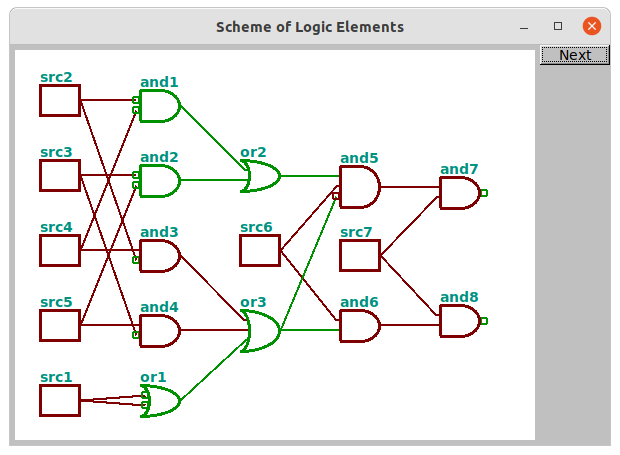
\includegraphics[width=0.6\textwidth]{images/logic_elements.png}

    }
    \caption{Пример рисования логической схемы}
    \label{fig:logicelems}
\end{figure}



%%========================
\paragraph{Анализ задачи.}
%%========================
Нам дан пример схемы с~логическими элементами. Нужно ответить на~следующие вопросы и сформулировать задачу.
\begin{enumerate}
    \item Какова предметная область?
    \begin{itemize}
        \item Работаем с~элементами математической логики.
    \end{itemize}

    \item В~каком контексте нужно разработать программный код?
    \begin{itemize}
        \item Необходим программный код, который позволяет смоделировать работу данной схемы.
        \item Этот код вполне вероятно будет использован для~моделирования подобных схем.
        \item Было бы удобно, если бы моделирование схемы не~зависело от~способа отображения процесса её работы (рисования).
    \end{itemize}

    \item Анализ исходных данных:
    \begin{itemize}
        \item На~схеме изображены не~все существующие логические элементы.
        \item На~схеме нет циклов.
        \item Вместо логического отрицания используются отрицания на~выходах/входах логических элементов.
    \end{itemize}
\end{enumerate}



%%=========================
\paragraph{Проектирование.}
%%=========================
Необходимо предусмотреть гибкость разрабатываемого программного кода.
\begin{itemize}
    \item Расширение функционала не~должно вынуждать полностью переписывать исходный код.
    \item Разделение на~небольшие части, подзадачи, которые могут быть использованы независимо (принцип <<разделяй и властвуй>>).
    \item Необходимо предусмотреть наиболее удобные уровни абстракции.
\end{itemize}

\bigskip Выделим в~коде две части:
\begin{itemize}
    \item Код для~непосредственного моделирования работы схемы.
    \item Код для~отображения процесса работы схемы (рисование).
\end{itemize}

\bigskip Продумаем примеры того, как бы мы хотели видеть использование разработанного программного кода:
\begin{enumerate}
    \item Создание элементов.
    \begin{itemize}
        \item При~создании логического элемента нужно указать его тип (тип объекта), инвертирован ли его выход (по~умолчанию не~инвертирован), задать \code{callback}-функцию (по~умолчанию \code{nullptr}).
        \item При~создании источника логического значения (сигнала) нужно указать это значение (по~умолчанию \code{false})
    \end{itemize}

    \item Соединение элементов.
    \begin{itemize}
        \item Соединений между логическими элементами гораздо больше, чем самих элементов.
        \item При~попытке сделать цикл в~схеме должно генерироваться исключение.
        \item Нужно предусмотреть (насколько это возможно) интуитивно понятный и лаконичный способ для~задания соединений.
        \item Удобно было бы соединять элементы по~цепочке.
        \item Будем использовать оператор \code{>>} для~соединения элементов (\code{and1 >> or2}).
        \item Подключение на~инвертированный вход вполне удобно смотрится с~использованием оператора~\code{\textasciitilde} (\code{or3 >> \textasciitilde{}and5}).
    \end{itemize}

    \item Изменение элементов.
    \begin{itemize}
        \item Для~задания логического значения источника удобно использовать оператор~\code{=}.
        \item Расчёт значений на~выходе каждого логического элемента должно происходить автоматически при~изменении состояния на~выходе элементов ниже по~цепочке.
        \item При~изменении состояния на~выходе элемента, этот элемент должен вызывать \code{callback}-функцию.
    \end{itemize}

    \item Получение значения на~выходе логического элемента.
    \begin{itemize}
        \item Оператор преобразования логического элемента в~значение \code{bool}.
    \end{itemize}

    \item Программный код для~отображения схемы и процесса её работы.
    \begin{enumerate}
        \item Нужно задавать только объекты, которые соответствуют логическим элементам на~схеме.
        \item Удобно создать класс-хранилище графических объектов SchemeShape.
        \item Отображение связей будет автоматическое, генерация объектов будет происходить в~SchemeShape.
        \item При~создании графических объектов нужно указать:
        \begin{itemize}
            \item на~какой схеме они расположены;
            \item какой логический элемент представляют;
            \item подпись (имя элемента);
            \item положение на~схеме.
        \end{itemize}
        \item Объект графического представления будет задавать \code{callback}-функцию для~элемента, который представляет.
        \item В~\code{callback}-функции будет происходить изменение цвета отображения элемента и связей.
    \end{enumerate}
\end{enumerate}



%%=========================================
\paragraph{Диаграмма наследования классов.}
%%=========================================
Набросаем иерархию классов которые будут воплощать логические элементы \todo{(нужно обновить)}.
\begin{center}\begin{tikzpicture}[node font=\ttfamily\small, >=Stealth]
    \graph [layered layout, components go right top aligned, edge=<-]
    {
        Shape[as=Graph\_lib::Shape] -> Element[align here, text=blue] ->[blue] {
            Source[text=blue],
            Operation[text=blue]
        };
        Operation ->[blue] {
            And[text=blue],
            Or[text=blue]
        };
        Board[text=blue];
    };

    \begin{scope}[on background layer]
        \node (Logic) [draw, blue, dashed, rounded corners,
        fit=(Element) (Source) (Board) (Operation) (And) (Or)] {};
        \node[text=blue, inner sep=0pt, above right=0pt of Logic.north east] {Logic};
    \end{scope}
\end{tikzpicture}\end{center}



%%=====================
\paragraph{Реализация.}
%%=====================
Объявление классов и констант разместим в~заголовочном файле \code{logic.h}, а реализацию методов "--- в~файле \code{logic.cpp}.

\todo{Дальнейшее описание будет размещено позднее.}



%%================
\WhatToReadSection
%%================
\textcite{Stroustrup:2016:ru}: \textbf{глава~10}



%%===============
\ExercisesSection
%%===============
\begin{exercise}
\item Выполните упражнения из~\textbookref{главы 9} учебника.

\end{exercise}
